\section{Zielsetzung}
\label{sec:Zielsetzung}
Ziel ist es Schwingungen ein einem gedämpften Schwingkreis und einem Serienresonanzkreis zu untersuchen und daraus
Ruckschlüsse auf den effektiven Wiederstand, den Wiederstand zum auftreten des aperiodischen Grenzfalls und der Frequenzabhängigkeit
im Serienresonanzkreis zu schließen.
\section{Theorie}
\label{sec:Theorie}
\subsection{Gedämpfte Schwingungen des RC-Kreises}
Der gedämpfte Schwingkreis ist aus einem Wiederstand $R$, einem Kondensator mit Kapazität $C$ und
einer Spule mit Induktivität $L$ wie in \autoref{abb:GedSchwing} dargestellt aufgebaut. Dabei schwingt
die zugeführte elektrische Energie zwischen der Spule und dem Kondensator. Durch den Wiederstand nimmt diese im zeitlichen
Verlauf ab und wird in Wärme umgewandelt, daher handelt es sich um eine gedämpfte Schwingung.
\begin{figure}[H]
    \centering
    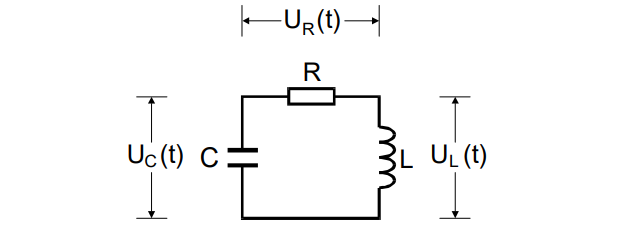
\includegraphics[scale=1]{content/GedSchwing.png}
    \caption{Der gedämpfte Schwingkreis. \cite{sample}}
    \label{abb:GedSchwing}
\end{figure}
\noindent Aus \autoref{abb:GedSchwing} folgt nach dem 2.Kirchhoffschen Gesetz
\begin{equation*}
    0 = U_R + U_C + U_L
\end{equation*}
für die Spannungen.
Daraus folgt die Differentialgleichung der gedämpften Schwingung
\begin{equation*}
    0 = \frac{d^2 I}{dt^2} + \frac{R}{L}\frac{dI}{dt} + \frac{1}{LC}I
\end{equation*}
mit der Lösung
\begin{equation}
    \label{eqn:AllgLoes}
    I(t) = e^{-2\pi\mu t}\left(U_1e^{i2\pi\nu t} + U_2e^{-i2\pi\nu t}\right).
\end{equation}
Dabei sind
\begin{align}
   2\pi\mu &= \frac{R_{Eff}}{2L}\\
   2\pi\nu &= \sqrt{\frac{1}{LC} - \frac{R^2}{4L^2}}
\end{align}
und $i$ die imaginäre Zahl.
Es wird bei $\nu$ zwischen zwei Spezialfällen unterschieden.\\
1. Fall: $\nu\in\mathbb{R}$\\
Hier folgt für die Lösung der Differentialgleichung
\begin{equation}
    I(t) = A_0e^{-2\pi\mu t}\cos(2\pi\nu t + \eta).
\end{equation}
Bei diesem Fall handelt es sich um den Schwingfall wie in \autoref{abb:Schwing} dargestellt und die Abklingdauer beträgt
\begin{equation}
    T_{ex} = \frac{R}{4\pi L}.
\end{equation}
\begin{figure}[H]
    \centering
    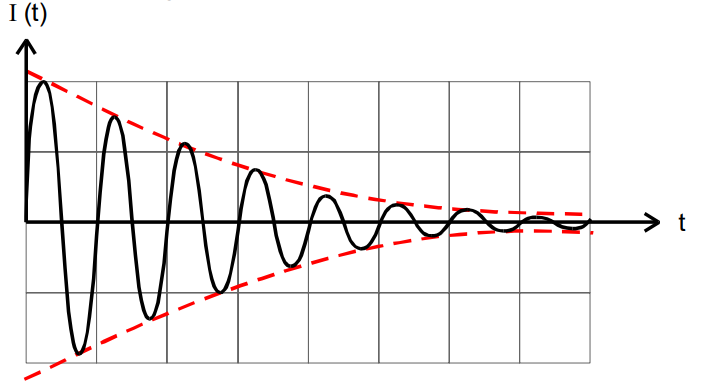
\includegraphics[scale=1]{content/Schwing.png}
    \caption{Der Schwingfall der gedämpften Schwingung mit der Einhüllenden $\pm e^{-2\pi\mu t}$. \cite{sample}}
    \label{abb:Schwing}
\end{figure}
\noindent 2. Fall: $\nu\in\mathbb{C}$\\
Bei diesem Fall enthält die Lösung $I(t)$ keinen oszillierenden Anteil und diese folgt einem Relaxationsverfahren.
Je nach wahl der Konstanten $U_1$ und $U_2$ aus \eqref{eqn:AllgLoes} liegen Extrema vor bis die Gleichung für große
$t$ gegen Null geht. Wenn $\nu = 0$ liegt der aperiodische Grenzfall vor, dargestellt durch die gestrichelte Kurve in
\autoref{abb:UberSchw}, wo die Kurve am schnellsten gegen Null fällt und keine Überschwingung vorliegt. Bei $\nu = 0$ gilt
$\frac{1}{LC} = \frac{R^2_{ap}}{4L^2}$ und für $I(t)$ gilt
\begin{equation}
    I(t) = Ae^{-\frac{t}{\sqrt{LC}}}.
\end{equation}
\begin{figure}[H]
    \centering
    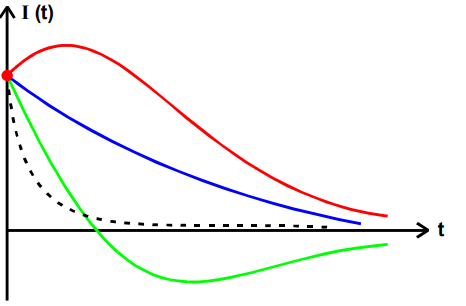
\includegraphics[scale=1]{content/UberSchw.png}
    \caption{Verlauf von $I(t)$ bei aperiodischer Dämpfung. \cite{sample}}
    \label{abb:UberSchw}
\end{figure}
\subsection{Erzwungene Schwingungen des RC-Kreises}
\begin{figure}[H]
    \centering
    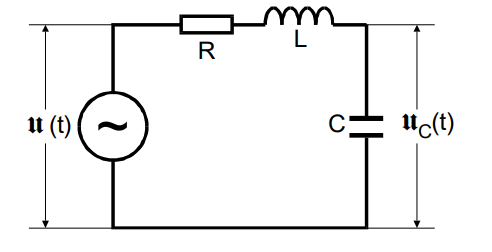
\includegraphics[scale=1]{content/ErzwSchwing.png}
    \caption{Schwingkreis der erzwungenen Schwingung mit sinusförmiger Erregerspannung. \cite{sample}}
    \label{abb:ErzwSchwing}
\end{figure}
Für die Differentialgleichung mit der Eingangsspannung $U_0$ folgt hier
\begin{equation}
    \label{eqn:ErzDGL}
    U(t) = U_0e^{i\omega t} = LC\frac{d^2U_C}{dt^2} + RC\frac{dU_C}{dt} + U_C
\end{equation}
mit
\begin{equation}
    \label{eqn:UC}
    U_C(\omega) = \frac{U_0}{\sqrt{\left(1-LC\omega^2\right)^2 + \omega^2R^2C^2}}.
\end{equation}
Für große Frequenzen geht die Spannungsamplitude $U_C$ gegen null und bei kleinen Frequenzen gegen $U_0$.
Es folgt ebenfalls aus \eqref{eqn:ErzDGL} folgt für die Phase $\varphi$
\begin{equation}
    \varphi(\omega) = \arctan\left(\frac{-\omega RC}{1-LC\omega^2}\right).
\end{equation}
Die Kondensatorspannung erreicht ein Maximum bei der Resonanzfrequenz $\omega_{res}$ nach
\begin{equation}
    \omega_{res} = \sqrt{\frac{1}{LC} - \frac{R^2}{2L^2}}.
\end{equation}
Im Fall der schwachen Dämpfung $\left(\frac{R^2}{2L^2}\ll \frac{1}{LC}\right)$ liegt das Maximum der Kondensatorspannung bei
\begin{equation}
    U_{C,\symbf{max}} = \frac{1}{\omega_0RC}U_0 = \frac{1}{R}\sqrt{\frac{L}{C}}U_0,
\end{equation}
wobei der Faktor $\frac{1}{\omega_0RC}$ auch als Güte $q$ des Schwingkreises bezeichnet.
Die schärfe der Resonanz lässt sich mit der Breite der Kurve aus \eqref{eqn:UC}. Diese wird charakerisiert
durch die Frequenzen $\omega_+$ und $\omega_-$ bei welchen die Spannung $U_C$ auf $\frac{1}{\sqrt{2}}$ des
Maximalwertes abgefallen ist. Die Güte $q$ lässt sich über die Breite der Resonanzkurve mit
\begin{equation}
    q = \frac{\omega_0}{\omega_+ - \omega_-}
\end{equation}
ausdrücken.
